\chapter{\selectlanguage{greek}Προσομοίωση \en{DVB-S2 RA} κώδικα σε κανάλι \en{AWGN}}
\externaldocument{chapter3.tex}
Στο κεφάλαιο αυτό, θα παρουσιαστεί ο δέκτης που προσομοιώθηκε και τα αποτελέσματα της προσομοίωσης σε καμπύλες \en{BER/FER} για τους διάφορους ρυθμούς που έχουν προτυποποιηθεί για την ψηφιακή τηλεόραση δεύτερης γενιάς (\en{DVB-S/T2}).

Αρχικά παρουσιάζεται συνοπτικά η διαμόρφωση \en{QPSK} και κατόπιν η διαδικασία αποδιαμόρφωσης (\en{demapping}), μέσω έτοιμων συναρτήσεων που παρέχονται από το \en{MATLAB}. Στη συνέχεια παρουσιάζεται το σύνολο της προσομοίωσης και στο τέλος του κεφαλαίου, τα αποτελέσματά της.

\section{\en{QPSK Demapper}}
\subsection{Διαμόρφωση \en{QPSK}}
Η κωδική λέξη, μετά την έξοδό της από τον κωδικοποιητή καναλιού, απεικονίζεται στον \en{QPSK} αστερισμό και προκύπτει η ακολουθία μιγαδικών σημάτων, μήκους $n/2$. Σε μορφή ημιτονοειδών κυμάτων μετάδοσης, ο \en{QPSK} αστερισμός γράφεται ως εξής:

\begin{equation}
s_n(t)=\sqrt{\frac{2E_s}{T_s}}\cos\left(2{\pi}f_ct+(2m-1)\frac{\pi}{4}\right),\;\;\;m=1,2,3,4.
\label{eq:QPSK sinusoid waves}
\end{equation}
όπου $E_s$ η ενέργεια συμβόλου, $T_s$ η περίοδος σηματοδοσίας, $f_c$ η συχνότητα του φέροντος κύματος και $m$ ο δείκτης των συμβόλων. Το αποτέλεσμα είναι ένας δι-διάστατος χώρος σημάτων με μοναδιαίες συναρτήσεις βάσης:

\begin{equation}
\begin{aligned}
\phi_1=\sqrt{\frac{2}{T_s}}\cos(2{\pi}f_ct) \\ \phi_2=\sqrt{\frac{2}{T_s}}\sin(2{\pi}f_ct)
\end{aligned}
\label{eq:QPSK base functions}
\end{equation}
όπου $\phi_1$ είναι η συμφασική και $\phi_2$ η ορθογώνια συνιστώσα. Το σήμα αποτυπώνεται στα 4 σημεία του αστερισμού \en{QPSK} $\left(\pm\sqrt{E_s/2},\pm\sqrt{E_s/2}\right)$ και οι φάσεις των συμβόλων προκύπτουν $\pi/4$, $3\pi/4$, $5\pi/4$ και $7\pi/4$. Ο παραπάνω αστερισμός φαίνεται στο Σχήμα \ref{fig:qpsk constellation}:

\begin{figure}[H]
\center{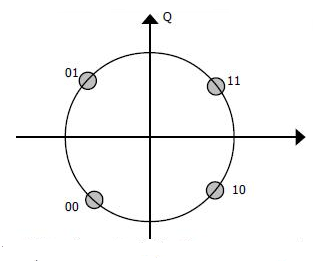
\includegraphics[width=0.55\linewidth]{figures/qpsk_constellation_diagram.png}}
\caption{Ο αστερισμός \en{QPSK}}
\label{fig:qpsk constellation}
\end{figure}
\hfill\\

Στη συνέχεια το σήμα περνάει από το κανάλι μετάδοσης, όπου προστίθεται το \en{AWGN} θόρυβος. Στο δέκτη ακολουθείται η αντίστροφη διαδικασία. Το \en{Matlab} παρέχει έτοιμη μέθοδο αποδιαμόρφωσης και ανίχνευσης μέσω του αντικειμένου \en{comm.QPSKDemodulator} και της μεθόδου \en{step}.

Το αντικείμενο αυτό δουλεύει ως εξής: μετά την έξοδο από το κανάλι η ακολουθία μιγαδικών αριθμών $\mathbf{y}$ μήκους $n/2$ εισάγεται στον \en{demapper}, ο οποίος παράγει μετρικές $L(x_{ij})$ στο διάστημα $(-\infty,\infty)$ για καθένα από τα κωδικά \en{bits} $x_{ij}$, σύμφωνα με τη σχέση:

\begin{equation}
L(x_{ij})=\ln\frac{p(x_{ij}=0\mid\mathbf{y}_i)}{p(x_{ij}=1\mid\mathbf{y}_i)},\;\;\;i\in\left[1,\frac{n}{2}\right],j=1,2.
\label{eq:QPSK LLR}
\end{equation}
οι οποίες εισάγονται στον επαναληπτικό αποκωδικοποιητή για την αρχικοποίησή του.

Από τις εξισώσεις \ref{eq:QPSK sinusoid waves}, \ref{eq:QPSK base functions} προκύπτει πως η διαμόρφωση \en{QPSK} αποτελεί απεικόνιση των δυάδων $\{0,1\}^2$, οι οποίες καλούνται \textit{ετικέτες} (\en{labels}), στο σύνολο των \en{QPSK} σημάτων $S$, δηλαδή $\{0,1\}^2\to{S}$. Αν συμβολιστεί ως ${S}_0^j$  το υποσύνολο των στοιχείων του $S$ που στην \en{j}-οστή θέση της ετικέτας τους έχουν 0 και ως ${S}_1^j$ το υποσύνολο των στοιχείων του $S$ που στην \en{j}-οστή θέση της ετικέτας τους έχουν 1 και θεωρηθεί απεικόνιση \en{Gray}, προκύπτουν σχηματικά τα υποσύνολα του Σχήματος \ref{fig:qpsk subtotals}.

\begin{figure}[H]
\center{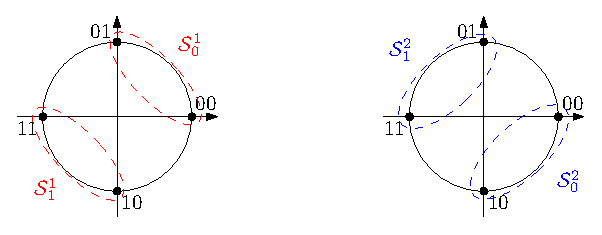
\includegraphics[width=0.55\linewidth]{figures/qpsk.eps}}
\caption{Τα υποσύνολα $ \color{red} {S}_1^0$, $ \color{red} {S}_1^1$ και $ \color{blue} {S}_0^0$, $ \color{blue}{S}_0^1$}
\label{fig:qpsk subtotals}
\end{figure}

Η σχέση \ref{eq:QPSK LLR} μπορεί να αναλυθεί περεταίρω για το κωδικό \en{bit} $L(x_{i1})$, αν εφαρμοστεί ο νόμος ολικής πιθανότητας, επιμερίζοντας σε όλα τα γεγονότα $x_{i2}$, το γεγονός $\{x_{i1}=0\}$ στον αριθμητή και το $\{x_{i1}=1\}$ στον παρονομαστή, ώστε να πάρει την μορφή της εξίσωσης \ref{eq:fraction 4.1}:

\begin{equation}
\begin{split}
L(x_{i1}) & =\ln\frac{\sum\nolimits_{x_{i2}}p(x_{i1}=0, x_{i2}\mid\mathbf{y}_i)}{\sum\nolimits_{x_{i2}}p(x_{i1}=1, x_{i2}\mid\mathbf{y}_i)} \\
& = \ln\frac{\sum\nolimits_{\mathbf{s}\in{S}_0^1} p(\mathbf{s}\mid\mathbf{y}_i)}{\sum\nolimits_{\mathbf{s}\in{S}_1^1} p(\mathbf{s}\mid\mathbf{y}_i)}
\end{split}
\label{eq:fraction 4.1}
\end{equation}

Γενικεύοντας από την εξίσωση \ref{eq:fraction 4.1}, για το κωδικό \en{bit} $L(x_{ij})$, προκύπτει:

\begin{equation}
\begin{split}
L(x_{ij}) & = \ln\frac{\sum\nolimits_{\mathbf{s}\in{S}_0^j} p(\mathbf{s}\mid\mathbf{y}_i)}{\sum\nolimits_{\mathbf{s}\in{S}_1^j} p(\mathbf{s}\mid\mathbf{y}_i)} \\
& = \ln\frac{\sum\nolimits_{\mathbf{s}\in{S}_0^j} p(\mathbf{y}_i\mid\mathbf{s})p(\mathbf{s})}{\sum\nolimits_{\mathbf{s}\in{S}_1^j} p(\mathbf{y}_i\mid\mathbf{s})p(\mathbf{s})} \\
& = \ln\frac{\sum\nolimits_{\mathbf{s}\in{S}_0^j} p(\mathbf{y}_i\mid\mathbf{s})}{\sum\nolimits_{\mathbf{s}\in{S}_1^j} p(\mathbf{y}_i\mid\mathbf{s})}
\end{split}
\label{eq:fraction 4.2}
\end{equation}

Οι ισότητες λογαρίθμων στην εξίσωση \ref{eq:fraction 4.2} προκύπτουν χρησιμοποιώντας τον κανόνα του \en{Bayes} και υποθέτοντας ότι τα σήματα $\mathbf{s} \in S$ είναι ισοπίθανα.

Ακόμη για το διακριτό κανάλι \en{AWGN}, η κατανομή πυκνότητας πιθανόητας $p(\mathbf{y}_i\mid\mathbf{s})$ ορίζεται ως εξής:

\begin{equation}
p(\mathbf{y}_i\mid\mathbf{s})=\frac{1}{2\pi\sigma^2}\exp\left\{-\frac{{\norm{\mathbf{y}_i-\mathbf{s}}}^{2}}{2\sigma^2}\right\}
\label{eq:AWGN pdf}
\end{equation}

Συνοψίζοντας, η εξίσωση \ref{eq:fraction 4.1}, λόγω των \ref{eq:fraction 4.2}, \ref{eq:AWGN pdf} γίνεται:

\begin{equation}
\begin{split}
L(x_{ij}) & =\ln \frac{\sum \nolimits_{\mathbf{s}\in{S}_0^j} \exp \left\{ -\frac{\norm{\mathbf{y}_i}^2 -2\Re(\mathbf{y}_i\cdot\mathbf{s}) + \norm{\mathbf{s}}^2}{2\sigma^2} \right\}}{\sum \nolimits_{\mathbf{s}\in{S}_1^j} \exp \left\{ -\frac{\norm{\mathbf{y}_i}^2 -2\Re(\mathbf{y}_i\cdot\mathbf{s}) + \norm{\mathbf{s}}^2}{2\sigma^2} \right\}} \\
& =\ln \frac{\sum \nolimits_{\mathbf{s}\in{S}_0^j} \exp \left\{ \frac{\Re(\mathbf{y}_i\cdot\mathbf{s})}{\sigma^2}\right\}}{\sum \nolimits_{\mathbf{s}\in{S}_1^j} \exp \left\{ \frac{\Re(\mathbf{y}_i\cdot\mathbf{s})}{\sigma^2}\right\}}
\end{split}
\label{eq:fraction 4.3}
\end{equation}

Στην εξίσωση \ref{eq:fraction 4.3}, θεωρώντας πως η ενέργεια σήματος $\norm{\mathbf{s}}^2=E_s,\;\forall \; \mathbf{s} \in S$ είναι η ίδια, οι παράγοντες $\exp\left\{-\frac{\norm{\mathbf{y}_i}^2}{2\sigma^2}\right\}$, $\exp\left\{-\frac{\norm{\mathbf{s}}^2}{2\sigma^2}\right\}$ μπορούν να απαλειφθούν με παραγοντοποίηση σε αριθμητή και παρονομαστή και τελικά η εξίσωση \ref{eq:fraction 4.3} να λάβει τη μορφή:

\begin{equation}
L(x_{ij})=\ln\frac{\sum \nolimits_{\mathbf{s}\in{S}_0^j}\exp\left\{\frac{y_{iI}s_I+y_{iQ}s_Q}{\sigma^2}\right\}}{\sum \nolimits_{\mathbf{s}\in{S}_1^j}\exp\left\{\frac{y_{iI}s_I+y_{iQ}s_Q}{\sigma^2}\right\}}
\label{eq:fraction 4.4}
\end{equation}
όπου οι δείκτες $I$, $Q$ υποδεικνύουν προβολή του αντίστοιχου διανύσματος στη συμφασική και στην ορθογώνια συνιστώσα αντίστοιχα.

\section{Προσομοίωση στο \en{Matlab}}
% \selectlanguage{english}
% {spa9.m}
% 
\begin{table}[h]
\centering
\begin{tabular}
{>{\bfseries}c*{2}{c}}\toprule\toprule{\en{Rate R}} & {$(E_b/N_0)_{soft}\;\;(dB)$}\\ \midrule
1/4&-0.793\\
1/3&-0.497\\
2/5&-0.236\\
1/2&0.187\\
3/5&0.682\\
2/3&1.059\\
3/4&1.626\\
4/5&2.039\\
9/10&3.199\\ \bottomrule\bottomrule
\end{tabular}
\caption{Χωρητικότητα ως \en{$E_b/N_0$} για τους ρυθμούς κώδικα της προσομοίωσης}
\label{table: EbN0 limits}
\end{table}

Στον πίνακα \ref{table: EbN0 limits}, φαίνεται το (θεωρητικό) κάτω όριο $E_b/N_0$ για τον κάθε ρυθμό κώδικα που προσομοιώνεται, το οποίο καλείται \textit{όριο κωδικοποίησης} και αντιστοιχεί σε διαμόρφωση \en{BPSK} ή \en{QPSK}. Η χωρητικότητα, όπως εκφράζεται από τα παραπάνω όρια για δεδομένο ρυθμό \en{R}, δίνει ένα κατώφλι \en{SNR} μετά από το οποίο και με τη χρήση κωδικοποίησης καναλιού, μπορεί να επιτευχθεί -θεωρητικά- αξιόπιστη επικοινωνία, σε διαφορετική περίπτωση η αξιοπιστία της οποίας είναι μη ελέγξιμη.

Για να υλοποιηθεί προσομοίωση στο \en{Matlab} μεταβάλλεται η μεταβλητή \en{R} η οποία αποθηκεύει το ρυθμό του κώδικα και ορίζεται ο \en{LDPC} κώδικας με βάση τον πίνακα $\mathbf{H}$. Κατόπιν αρχικοποιούνται τα αντικείμενα που ορίζουν τις παραμέτρους της διαμόρφωσης-αποδιαμόρφωσης και κωδικοποίησης-αποκωδικοποίησης.

\tl{\lstinputlisting{def.m}}
\tl{\lstinputlisting{encdec.m}}
\tl{\lstinputlisting{moddemod.m}}

Η κωδικοποίηση γίνεται σύμφωνα με όσα αναφέρθηκαν στο Κεφάλαιο 3 και ακολουθεί την συστηματική \en{LDPC}, σύμφωνα με το πρότυπο \en{Digital Video Broadcasting \& Satellite - Second Generation (DVB-S2)} \cite{etsi2009302}. Όπως φαίνεται από το παραπάνω κομμάτι κώδικα, το αντικείμενο \textit{\en{enc}} αρχικοποιείται με βάσει τον πίνακα ελέγου ισοτιμίας για δεδομένο ρυθμό κώδικα. Διακρίνεται από τα εξής βήματα:

\begin{itemize}
\item Αρχικοποίηση των \en{parity bits}: $p_0=p_1=\cdots=p_{n-k-1}=0$
\item Συσσώρευση του πρώτου \en{info bit} στις διευθύνσεις που δίνονται από την πρώτη γραμμή των πινάκων \en{B.1} έως \en{B.11} του παραρτήματος Β στο πρότυπο \en{ETSI} για το \en{DVB-S2} \cite{etsi2009302}, με \en{mod}-2 πρόσθεση.
\item Για τα επόμενα 359 \en{info bits} οι διευθύνσεις των συσσωρευτών δίνονται από τον τύπο $\lbrace x+\left(m\; mod\; 360\right) \times q\rbrace mod \left(n-k\right)$, όπου $m=1,2,\cdots,359$, το $x$ αντιστοιχεί στη διεύθυνση συσσωρευτή του πρώτου \en{info bit} και το $q$ δίνεται από τον Πίνακα \ref{table:q values}
\item Αντίστοιχα, για κάθε επόμενο \en{group} από 360 \en{info bits} χρησιμοποιείται μια καινούργια γραμμή διευθύνσεων στους πίνακες \en{B.1} έως \en{B.11} του παραρτήματος Β του \cite{etsi2009302}
\item Με την εξάντληση των \en{info bits}, τα τελικά \en{parity bits} $p_i$ δίνονται ως εξής:
\begin{equation*}
p_0 = p_0
\end{equation*}
\begin{equation*}
p_i = p_i \oplus p_{i-1},\;\;i=1,2,\cdots,n-k
\end{equation*}
\end{itemize}

\begin{table}[H]
\centering
\begin{tabular}
{>{\bfseries}c*{2}{c}}\toprule\toprule{\en{Code Rate}} & {$q$}\\ \midrule
1/4&135\\
1/3&120\\
2/5&108\\
1/2&90\\
3/5&72\\
2/3&60\\
3/4&45\\
4/5&36\\
9/10&18\\ \bottomrule\bottomrule
\end{tabular}
\caption{Τιμές $q$ για τους διάφορους ρυθμούς κώδικα της προσομοίωσης}
\label{table:q values}
\end{table}

Αντίστοιχα η αποκωδικοποίηση στηρίζεται στην εφαρμογή του \en{SPA} αλγορίθμου για \en{LDPC} και ακολουθεί την παρακάτω πορεία:

\begin{itemize}
\item Η αρχικοποίηση των $L_j$ γινεται μέσω της σχέσης \ref{eq:fraction 4.4}
\item Τα μηνύματα που εξέρχονται απο τους \en{CN} υπολογίζονται από την εξίσωση 
\begin{equation}
L_{i\to j} = 2\tanh^{-1} \left( \prod_{j'\in N(i)-\lbrace j\rbrace} \tanh \left( \frac{1}{2}L_{j'\to i} \right)\right)
\end{equation}
και κατόπιν μεταδίδονται στους \en{VN}
\item Τα μηνύματα που εξέρχονται απο τους \en{VN} υπολογίζονται από την εξίσωση
\begin{equation*}
L_{j\to i} = L_j + \sum_{i'\in N(j)-\lbrace i\rbrace} L_{i'\to j}
\end{equation*}
και κατόπιν μεταδίδονται στους \en{CN}
\item Τα συνολικα \en{LLR} υπολογίζονται από τη σχέση
\begin{equation*}
L_{j}^{total} = L_j + \sum_{i\in N(j)} L_{i\to j}
\end{equation*}
\item Για $j=0,1,\cdots,n-1$ υπολογίζονται οι τιμές των \en{bit}
\begin{equation*}
\hat{v_j}=\left\{
\begin{array}{c l}	
     1 & L_{j}^{total}<0\\
     0 & else
\end{array}\right.
\end{equation*}
που διαμορφώνουν την $\hat{\mathbf{v}}$. Αν $\hat{\mathbf{v}}\mathbf{Η}=\mathbf{0}$, ο αλγόριθμος τερματίζει, αλλιώς συνεχίζει με την επόμενη επανάληψη.
\item Στο τέλος της προσομοίωσης υπολογίζονται οι μετρικές \en{BER} και \en{FER} για την προσομοίωση του εκάστοτε ρυθμού στο αντίστοιχο \en{SNR}
\end{itemize}


Η προσομοίωση έχει ως όριο τα $10^3$ σφάλματα ή τις $10^6$ προσπάθειες (\en{trials}) να εντοπιστούν. Τα αποτελέσματα που θα παρουσιαστούν, λαμβάνονται αφού αποθηκευτούν για κάθε ρυθμό το \en{Bit Error Rate - BER} και το \en{Frame Error Rate - FER}.

\section{Αποτελέσματα - Σχολιασμός}

Σε αυτό το σημείο παρουσιάζονται τα αποτελέσματα της προσομοίωσης. Τα διαγράμματα που ακολουθούν απεικονίζουν για κάθε ρυθμό του Πίνακα \ref{table: EbN0 limits} τις τιμές του \en{BER}, ξεκινώντας από την τιμή $E_b/N_0$ του Πίνακα \ref{table: EbN0 limits} (θεωρητικό όριο χωρητικότητας για κάθε ρυθμό) και καταλήγοντας στη τιμή $E_b/N_0$, για την οποία το \en{BER} φτάνει στο $10^{-8}$. Στα ίδια διαγράμματα απεικονίζονται και οι τιμές \en{FER} για τις αντίστοιχες τιμές $E_b/N_0$. Στο τέλος, δίνεται επίσης ένα συγκριτικό διάγραμμα όλων των καμπυλών \en{BER} και \en{FER}, για καλύτερη εποπτεία των αποτελεσμάτων των διαφόρων ρυθμών.
\begin{figure}[H]
\center{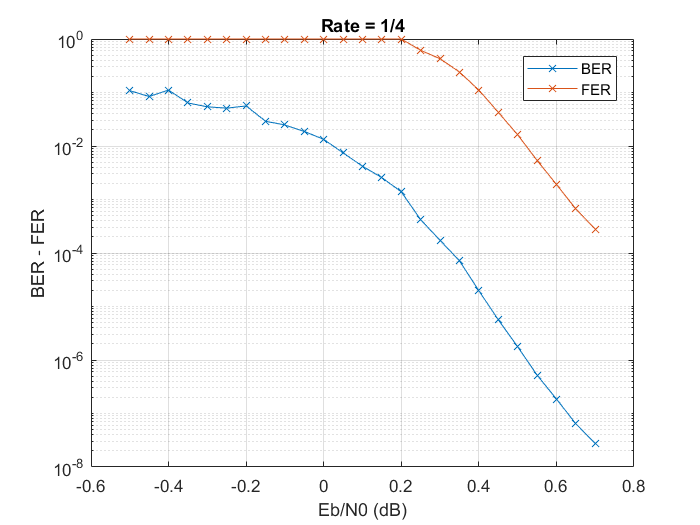
\includegraphics[width=0.75\linewidth]{matlab/1-4.png}}
\caption{\en{BER},\en{FER vs} $E_b/N_0$ για ρυθμό 1/4}
\end{figure}
\begin{figure}[H]
\center{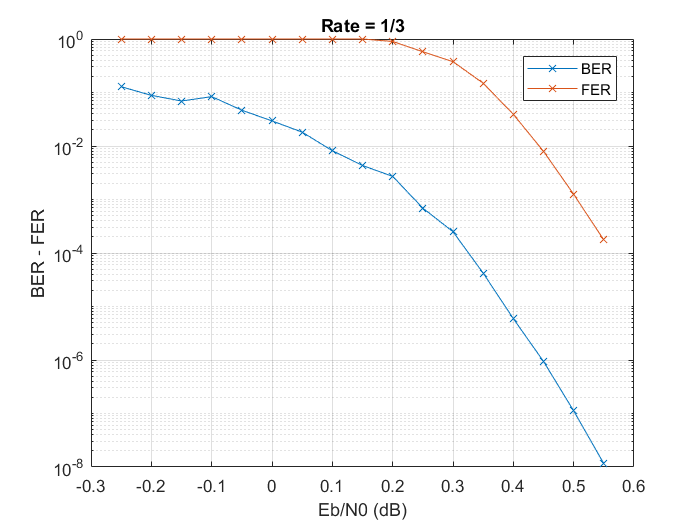
\includegraphics[width=0.75\linewidth]{matlab/1-3.png}}
\caption{\en{BER},\en{FER vs} $E_b/N_0$ για ρυθμό 1/3}
\end{figure}
\begin{figure}[H]
\center{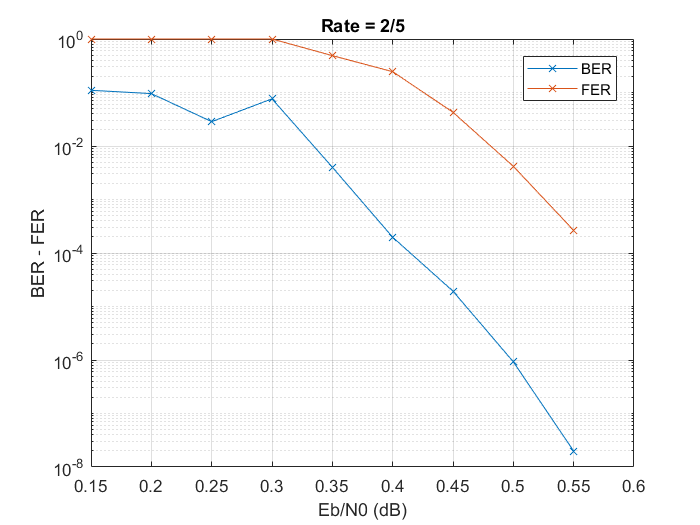
\includegraphics[width=0.75\linewidth]{matlab/2-5.png}}
\caption{\en{BER},\en{FER vs} $E_b/N_0$ για ρυθμό 2/5}
\end{figure}
\begin{figure}[H]
\center{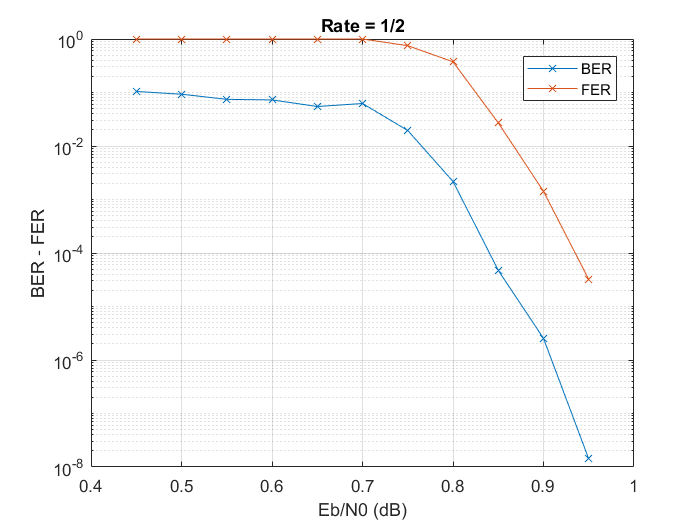
\includegraphics[width=0.75\linewidth]{matlab/1-2.png}}
\caption{\en{BER},\en{FER vs} $E_b/N_0$ για ρυθμό 1/2}
\end{figure}
\begin{figure}[H]
\center{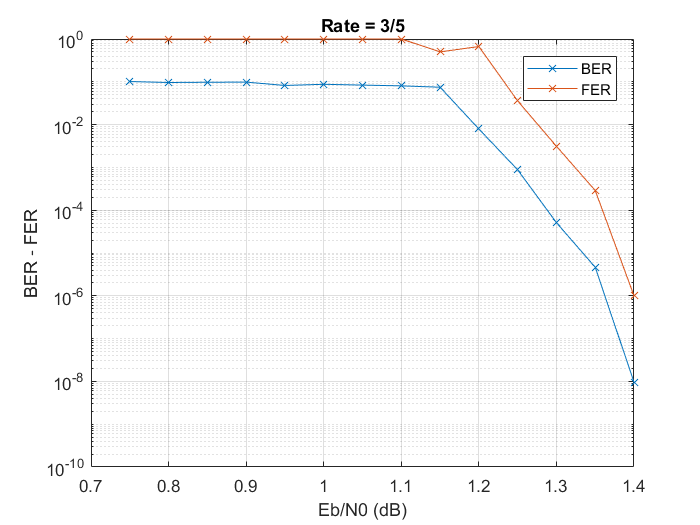
\includegraphics[width=0.75\linewidth]{matlab/3-5.png}}
\caption{\en{BER},\en{FER vs} $E_b/N_0$ για ρυθμό 3/5}
\end{figure}
\begin{figure}[H]
\center{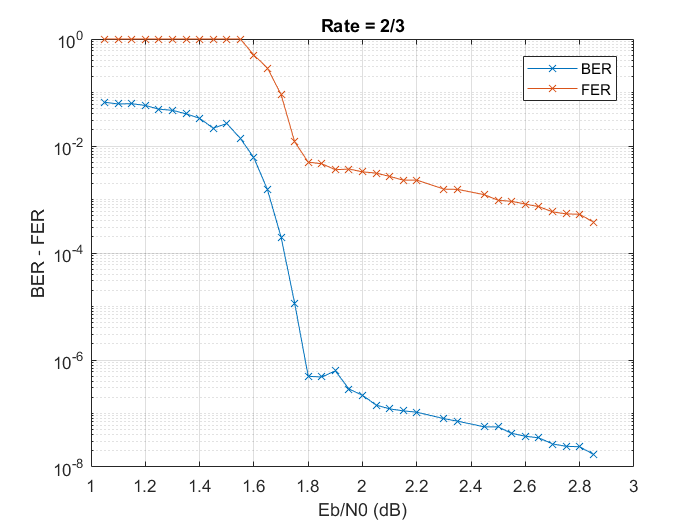
\includegraphics[width=0.75\linewidth]{matlab/2-3.png}}
\caption{\en{BER},\en{FER vs} $E_b/N_0$ για ρυθμό 2/3}
\end{figure}
\begin{figure}[H]
\center{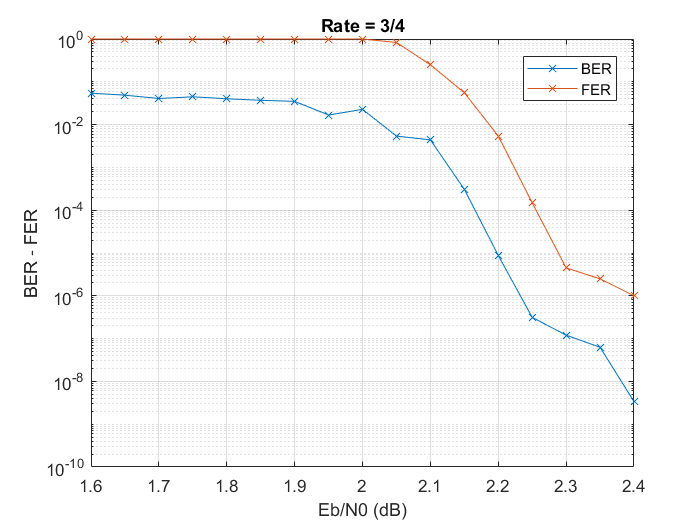
\includegraphics[width=0.75\linewidth]{matlab/3-4.png}}
\caption{\en{BER},\en{FER vs} $E_b/N_0$ για ρυθμό 3/4}
\end{figure}
\begin{figure}[H]
\center{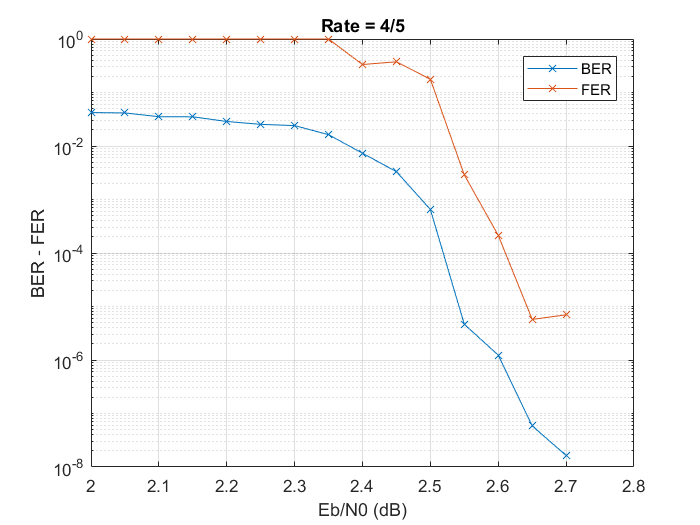
\includegraphics[width=0.75\linewidth]{matlab/4-5.png}}
\caption{\en{BER},\en{FER vs} $E_b/N_0$ για ρυθμό 4/5}
\end{figure}
\begin{figure}[H]
\center{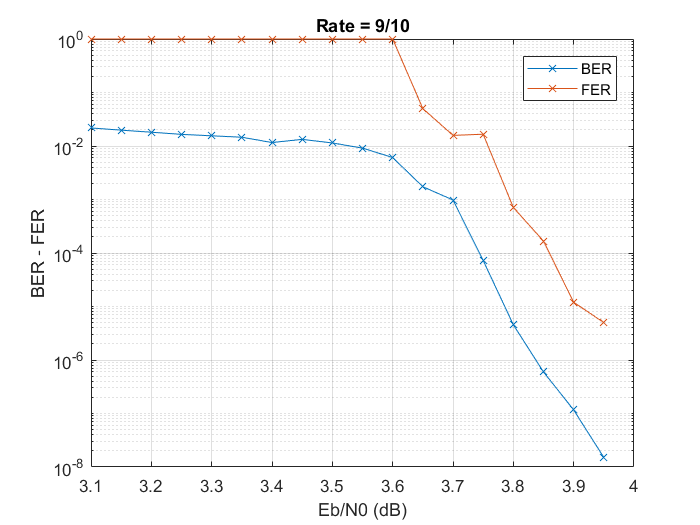
\includegraphics[width=0.75\linewidth]{matlab/9-10.png}}
\caption{\en{BER},\en{FER vs} $E_b/N_0$ για ρυθμό 9/10}
\end{figure}

\begin{figure}[H]
\center{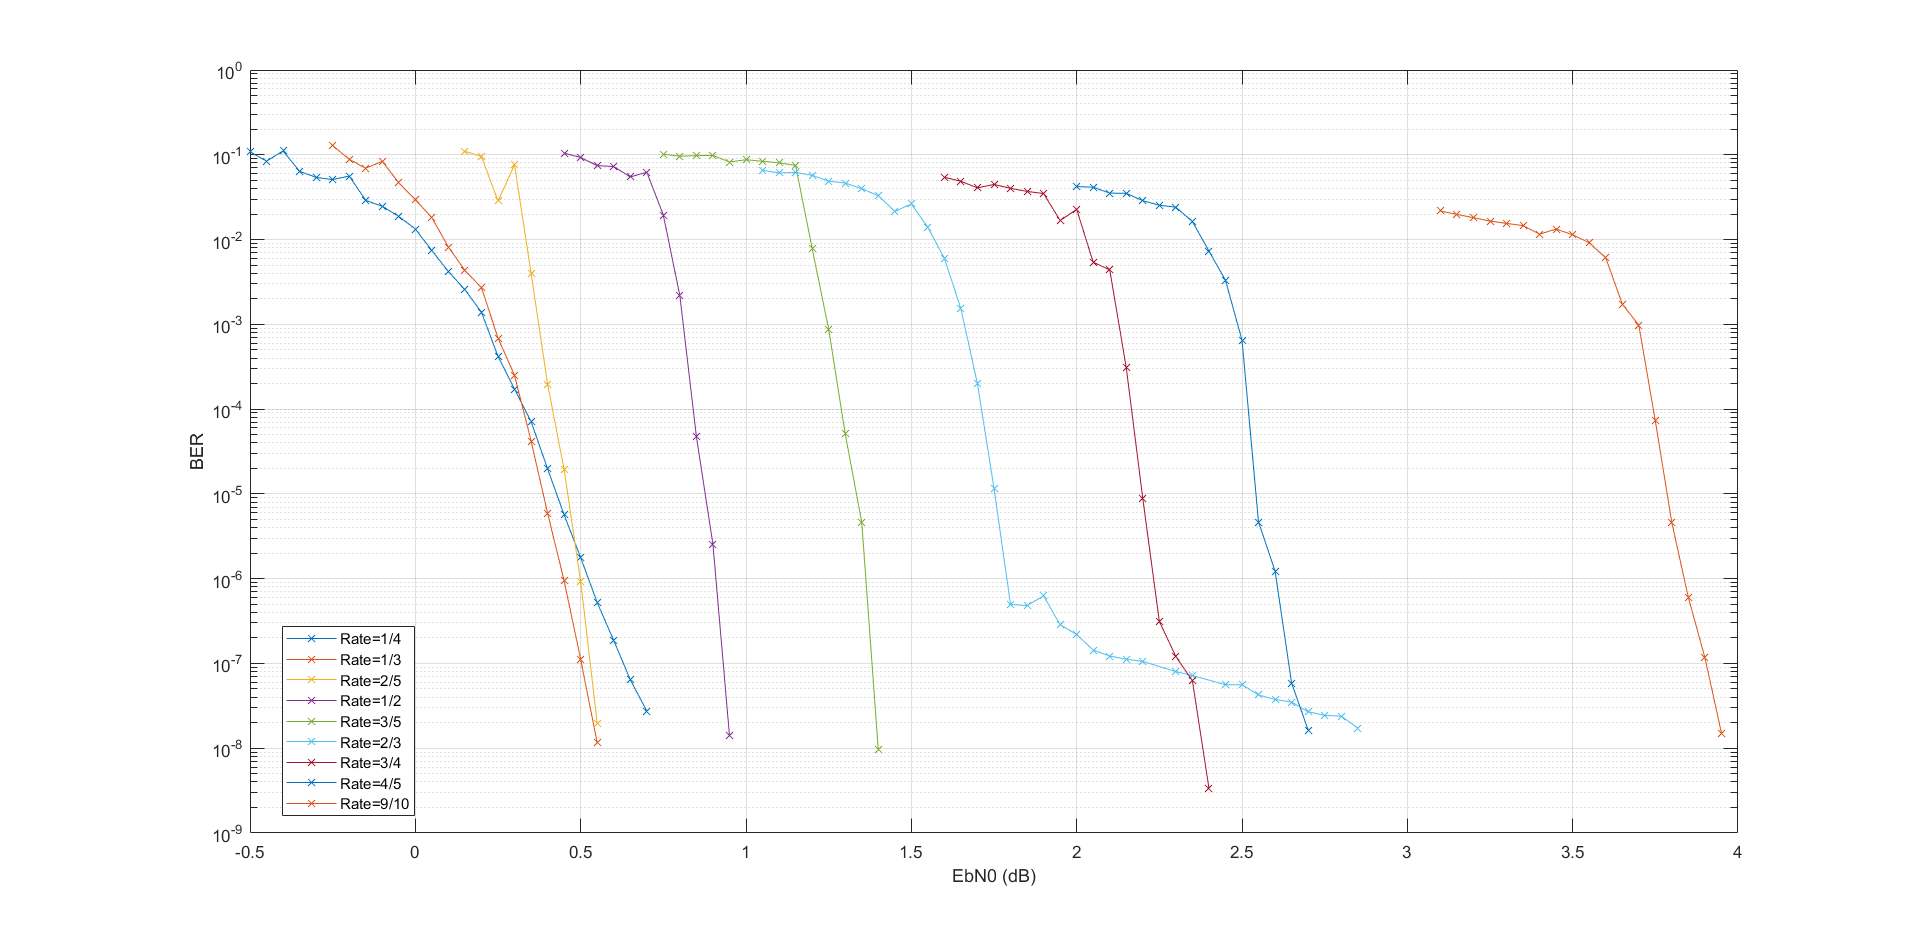
\includegraphics[width=1.0\linewidth]{matlab/full_BER.png}}
\caption{Καμπύλες \en{BER vs} $E_b/N_0$ για διαφορετικούς ρυθμούς}
\end{figure}

\begin{figure}[H]
\center{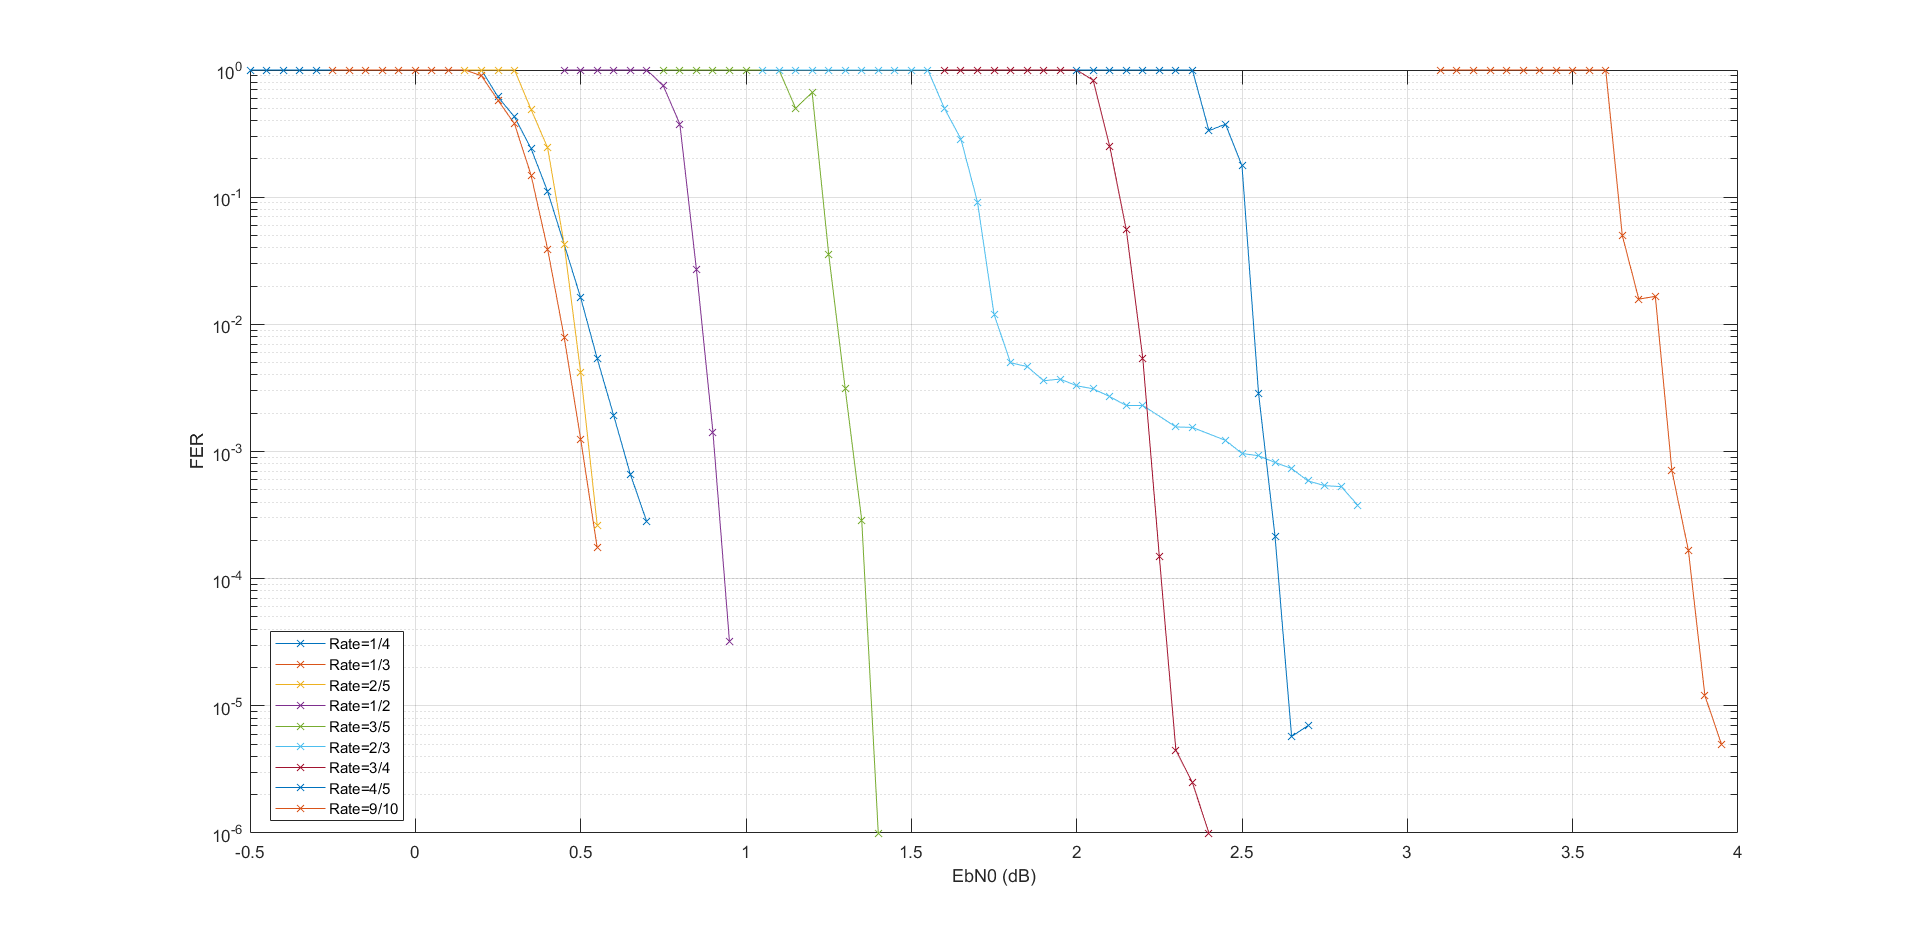
\includegraphics[width=1.0\linewidth]{matlab/full_FER.png}}
\caption{Καμπύλες \en{FER vs} $E_b/N_0$ για διαφορετικούς ρυθμούς}
\end{figure}

\subsection{Σχολιασμός}
Αρχικά παρατηρείται πως οι καμπύλες δεν είναι όσο λείες θα επιθυμούσαμε. Αυτό οφείλεται στον αριθμό των λαθών στα οποία σταματούσαμε την προσομοίωση, και ο οποίος σε κάποιες περιπτώσεις θα έπρεπε να είναι μεγαλύτερος. Αυτό θα βελτίωνε την αξιοπιστία της αντίστοιχης μέτρησης.

Ακόμη εντυπωσιάζει σε κάθε περίπτωση το ότι με πολύ μικρή αύξηση του \en{SNR}  βελτιώνεται ραγδαία ο ρυθμός σφαλμάτων. Επίσης, για όλους τους ρυθμούς επιβεβαιώνεται το γεγονός πως οι \en{RA} κώδικες του προτύπου \en{DVB-S2} είναι \en{capacity-approaching} κώδικες, μιας και μιας και απέχουν από τις χωρητικότητές τους απόσταση μικρότερη του 1 \en{dB}. Η μόνη περίπτωση στην οποία αυτό δεν ισχύει, είναι στον κώδικα με ρυθμό 1/4.

Τέλος, παρατηρούμε το έντονο \en{error-floor} του κώδικα ρυθμού 2/3 για τιμές του \en{BER} απο $10^{-6}$ και μετά. Φαινόμενα σαν κι αυτό επιλύονται με τη σειριακή αλύσωση του \en{RA} κώδικα με έναν εξωτερικό, κάτι που πράγματι συμβαίνει στο πρότυπο \en{DVB-S2}, όπου αυτός ο εξωτερικός είναι ένας \en{BCH} κώδικας.
